\documentclass[tikz,border=6pt]{standalone}
\usepackage{amsmath}
\usepackage{xcolor}
\usetikzlibrary{arrows.meta,positioning}

\definecolor{blockblue}{HTML}{4A90D9}
\definecolor{linegray}{HTML}{333333}

\begin{document}
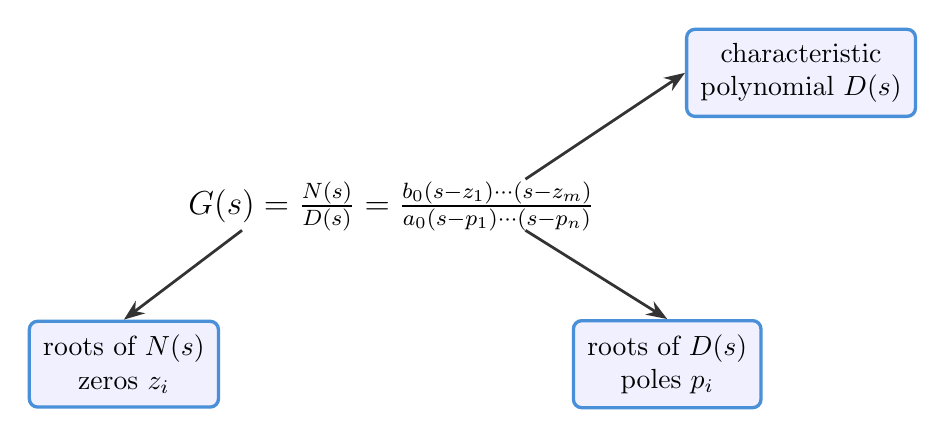
\begin{tikzpicture}[
  >=Stealth,
  line width=1.2pt,
  callout/.style={draw=blockblue, rounded corners=3pt, align=center, fill=blue!6, inner sep=5pt},
  flow/.style={->, draw=linegray, line width=1.0pt}
]
  \node[font=\large] (eq) at (0,0) {$
    G(s)=\frac{N(s)}{D(s)}
    =
    \frac{b_0(s-z_1)\cdots(s-z_m)}
    {a_0(s-p_1)\cdots(s-p_n)}
  $};

  \node[callout] (z) at (-3.4,-2.0) {roots of $N(s)$\\zeros $z_i$};
  \node[callout] (p) at (3.5,-2.0) {roots of $D(s)$\\poles $p_i$};
  \node[callout] (d) at (5.2,1.7) {characteristic\\polynomial $D(s)$};

  \draw[flow] (-1.9,-0.3) -- (z.north);
  \draw[flow] (1.7,-0.3) -- (p.north);
  \draw[flow] (1.7,0.35) -- (d.west);
\end{tikzpicture}
\end{document}
